\documentclass[12pt]{article}
\usepackage{fullpage}
\usepackage[titletoc,toc,page]{appendix}
\usepackage{setspace}
\usepackage{titlesec}
\usepackage{blindtext}
\usepackage{graphicx}
\usepackage{amssymb}
\usepackage{listings}
\usepackage{wrapfig}
\usepackage{xcolor}
\usepackage[main=greek, english]{babel}
\usepackage[utf8]{inputenc}
\usepackage[labelfont=bf]{caption}
\usepackage{kerkis}
\usepackage{url}
\usepackage{multicol}
\usepackage[titles]{tocloft}
\usepackage[top=2.5cm, bottom=2.5cm, left=2.8cm, right=3cm]{geometry}

\renewcommand\cftsecfont{\normalfont}
\renewcommand\cftsecpagefont{\normalfont}

\newcommand{\en}[1]{\foreignlanguage{english}{#1}}
\newcommand{\el}[1]{\selectlanguage{greek}{#1}\selectlanguage{english}}

\renewcommand\lstlistingname{\el{Συμβ.}}
\renewcommand\lstlistlistingname{Λίστα Συμβολισμών}
\setlength{\columnsep}{1cm}

\graphicspath{ {./images/} }
\setcounter{secnumdepth}{4}



\titlespacing*{\subsection}
{0pt}{2.5ex plus 1ex minus .2ex}{0.3ex plus .2ex}
\titlespacing*{\subsubsection}
{0pt}{2.5ex plus 1ex minus .2ex}{0.3ex plus .2ex}
\pagenumbering{gobble}

\begin{document}
 \begin{center}
\selectlanguage{greek}

\textsc{ ΠΑΝΕΠΙΣΤΗΜΙΟ ΜΑΚΕΔΟΝΙΑΣ\\[0.3 cm]
ΠΡΟΓΡΑΜΜΑ ΜΕΤΑΠΤΥΧΙΑΚΩΝ ΣΠΟΥΔΩΝ\\[0.3 cm]
ΤΜΗΜΑΤΟΣ ΕΦΑΡΜΟΣΜΕΝΗΣ ΠΛΗΡΟΦΟΡΙΚΗΣ}\\[2.5 cm]
{ \large 
ΠΑΡΑΛΛΗΛΟΣ ΠΡΟΓΡΑΜΜΑΤΙΣΜΟΣ ΜΕ ΧΡΗΣΗ \en{OpenMP}\\[0.4 cm] }
Διπλωματική Εργασία\\[1 cm]
του\\[0.5 cm]
\large
Κοντογιάννη Γεώργιου
\begin{minipage}{0.4\textwidth}
\end{minipage}
\vfill
{\large Θεσσαλονίκη, Οκτώβριος 2020}

 \end{center}
 
\pagenumbering{gobble}
\newpage
\mbox{}


\newpage
\pagenumbering{roman}
\setcounter{page}{3} 

 \begin{center}
{\large {ΠΑΡΑΛΛΗΛΟΣ ΠΡΟΓΡΑΜΜΑΤΙΣΜΟΣ ΜΕ ΧΡΗΣΗ \en{OpenMP}}}\\[2 cm]
Κοντογιάννης Γεώργιος\\[0.5 cm]
Δίπλωμα Πολιτικού Μηχανικού, ΑΠΘ, 2016\\[2 cm]
Διπλωματική Εργασία\\[0.5 cm]
υποβαλλόμενη για τη μερική εκπλήρωση των απαιτήσεων του\\[0.5 cm]
ΜΕΤΑΠΤΥΧΙΑΚΟΥ ΤΙΤΛΟΥ ΣΠΟΥΔΩΝ ΣΤΗΝ ΕΦΑΡΜΟΣΜΕΝΗ ΠΛΗΡΟΦΟΡΙΚΗ\\[2 cm]
\begin{flushleft}
Επιβλέπων Καθηγητής\\
Μαργαρίτης Κωνσταντίνος
\vfill
Εγκρίθηκε από την τριμελή εξεταστική επιτροπή την ηη/μμ/εεεε\\[0.5 cm]
\begin{tabular}{  p{\dimexpr 0.3333\linewidth-2\tabcolsep} 
                   p{\dimexpr 0.3333\linewidth-2\tabcolsep} 
                   p{\dimexpr 0.3333\linewidth-2\tabcolsep}  }
Ονοματεπώνυμο 1 & Ονοματεπώνυμο 2  & Ονοματεπώνυμο 3 \\[1 cm]
\dotfill & \dotfill  & \dotfill \\
\end{tabular}\\[2 cm]
Κοντογιάννης Γεώργιος \\[0.5 cm]
\begin{tabular}{  p{\dimexpr 0.3333\linewidth-2\tabcolsep}   }
\dotfill
\end{tabular}\\[1 cm]
\end{flushleft}
\end{center}
  
\setstretch{1.5}

\clearpage
\begin{small}
\begin{flushleft}
\
\vfil
\emph{Η σύνταξη της παρούσας εργασίας έγινε στο   \begin{LARGE}\en{\LaTeX}\end{LARGE}}
\end{flushleft}
\vfil
\end{small}



\clearpage
\begin{flushleft}
{\large \textbf{Περίληψη}}\\[0.5 cm]
\end{flushleft}

\subparagraph{}
Αντικείμενο της παρούσας διπλωματικής εργασίας είναι η μελέτη του \en{OpenMP}, ενός πρότυπου παράλληλου προγραμματισμού, που δίνει στο χρήστη τη δυνατότητα αναπτύξης παράλληλων προγραμμάτων για συστήματα μοιραζόμενης μνήμης, τα οποία  είναι ανεξάρτητα από τη συγκεκριμένη αρχιτεκτονική και έχουν μεγάλη ικανότητα κλιμάκωσης\cite{pdplab}.

Σκοπός της εργασίας είναι η μελέτη και συνοπτική περιγραφή των κύριων χαρακτηριστικών του \en{OpenMP 2.5} αλλά και των νεότερων εκδόσεων 3.0 και 4.5 και η υλοποίηση αλγορίθμων σειριακά και παράλληλα εκτελέσιμων, με σκοπό τη συγκριτική μελέτη της απόδοσής τους. Για την παράλληλη υλοποίηση θα γίνει χρήση της Διεπαφής Προγραμματισμού Εφαρμογών \en{(Application Programming Interface {-} API) OpenMP}, με χαρακτηριστικά που εισήχθησαν στις εκδόσεις \en{OpenMP} 3.0 που δημοσιεύθηκε το 2008 και \en{OpenMP} 4.5 που δημοσιεύθηκε 2015. Χρησιμοποιήθηκαν επίσης χαρακτηριστικά παλαιότερων εκδόσεων\cite{thenextstep59}.

Τον Μαιο του 2008 κυκλοφόρησαν οι προδιαγραφές του \en{OpenMP} 3.0 με την εισαγωγή των διεργασιών \en{(Tasking)} αλλά και βελτιώσεις στη \en{C++}. Αυτή ήταν η πρώτη ενημέρωση από την έκδοση 2.5 με σημαντικές βελτιώσεις. Το 2011 κυκλοφόρησε το \en{OpenMP} 3.1 χωρίς καινούργιο χαρακτηριστικά. Νέα λειτουργικότητα υλοποιήθηκε στο \en{OpenMP} 4.0 που κυκλοφόρησε τον Ιούλιο του 2013, όπου έγινε υποστήριξη της αρχιτεκτονικής \en{cc-NUMA}, του ετερογενούς προγραμματισμού, της διαχείρισης σφαλμάτων στο μπλοκ παράλληλου κώδικα και της διανυσματικοποίησης μέσω \en{SIMD}. Τον Ιούλιο του 2015 σημαντική βελτίωση έγινε στα παραπάνω χαρακτηριστικά με την έκδοση \en{OpenMP} 4.5\cite{thenextstep20}.

Τα προαναφερθέντα χαρακτηριστικά χρησιμοποιήθηκαν για την υλοποίηση των αλγορίθμων 
με διαφορετικές εναλλακτικές μεθόδους, με στόχο τη συγκριτική μελέτη τους για την εξαγωγή συμπερασμάτων αναφορικά με τη βελτίωση της απόδοσης σε σχέση με τη σειριακή υλοποίηση αλλά και τη μεταξύ τους σύγκριση καθώς επίσης, και αξιολόγηση της ευχρηστίας της υλοποίησής τους. Στόχος της έρευνας είναι να βρεθούν οι καλύτερες υλοποιήσεις των αλγορίθμων με την επίτευξη της μέγιστης αξιοποίησης της χρήσης \en{CPU} και/ή \en{GPU}. Ακόμη, γίνεται καταγραφή και αναφορά των προβλημάτων που μπορεί να προκύψουν για κάποια υλοποίηση.

Για την παραλληλοποίηση κώδικα, απαιτείται η σχεδίαση με τέτοιο τρόπο ώστε να παράγεται ένας μεγάλος αριθμός παράλληλων λειτουργιών που εκτελούνται από διαφορετικούς επεξεργαστές. Οι  αλγόριθμοι που χρησιμοποιήθηκαν στην παρούσα εργασία περιέχουν ένα μεγάλο αριθμών λειτουργιών, ικανών να εκτελεστούν παράλληλα. 

Τα βασικότερα παραδείγματα που χρησιμοποιήθηκαν είναι:
\begin{itemize}
    \item μετασχηματισμός \en{Fourier}, 
    \item \en{mergesort},
    \item υπολογισμός $\pi$, 
    \item πολλαπλασιασμός πινάκων,
    \item απλή εξίσωση διάδοσης θερμότητας,
    \item παραγοντοποίηση \en{cholensky}.
\end{itemize}

      
Για να υπάρχει άμεση σύγκριση των αποτελεσμάτων ο βασικός κορμός υλοποίησης είναι ο ίδιος για κάθε εφαρμογή, και οι χρονικές καταγραφές έγιναν σε συγκεκριμένα τμήματα του κώδικα. Οι παραλλαγές του κάθε αλγόριθμοι χρησιμοποιούν την \en{CPU} με απλή εκτέλεση χωρίς παραλληλοποίηση και με παράλληλη εκτέλεση. Οπου είναι εφικτό ο αλγόριθμους υλοποιείται  για εκτέλεση στην \en{GPU} για την επίλυση του. Οι χρονικές καταγραφές συγκρίνονται μεταξύ τους για την εξαγωγή συμπερασμάτων. Ακόμη, γίνεται αξιολόγηση της ευχρηστίας για την υλοποίηση της κάθε παραλλαγής αλλά και προβλημάτων που προέκυψαν.\\[1 cm]

\indent \textbf{Λέξεις Κλειδιά:}
Παράλληλος Προγραμματισμός, Παραλληλοποίηση, \en{OpenMP, accelerators, offloading, vectorization, SIMD, OpenMP4.5, UDRs}

\clearpage
\selectlanguage{english}
\begin{flushleft}

{\large \textbf{Abstract}}\\[0.5 cm]
\end{flushleft}
[Enter abstract here.]\\[1 cm]
\indent \textbf{Keywords:}

\clearpage
\selectlanguage{greek}
\begin{flushleft}
{\large \textbf{Ευχαριστίες}}\\[0.5 cm]
\end{flushleft}
\subparagraph{}
Εκφράζω τις θερμές μου ευχαριστίες στον επιβλέποντα καθηγητή κ. Κωνσταντίνο Μαργαρίτη, για την ουσιαστική του συνεισφορά στην εκπόνηση της παρούσας εργασίας.

\clearpage
\singlespacing
\tableofcontents
\setstretch{1.5}

\selectlanguage{greek}
\renewcommand{\listfigurename}{Κατάλογος Εικόνων (αν υπάρχουν)}
\clearpage
\listoffigures

\selectlanguage{greek}
\renewcommand{\listtablename}{Κατάλογος Πινάκων (αν υπάρχουν)}
\clearpage
\listoftables

\clearpage
\begin{flushleft}
\lstlistoflistings
\end{flushleft}

\clearpage
\setcounter{page}{1}
\pagenumbering{arabic}

\section{Εισαγωγή}
\subsection{Συνοπτικά για το \en{OpenMP}}
\subparagraph{}
Το \en{OpenMP} είναι μια Διεπαφή Προγραμματισμού Εφαρμογών \en{(API)} για παραλληλοποίηση συστημάτων μοιραζόμενης μνήμης, σε γλώσσες \en{C/C++} και \en{Fortran}. Η διεπαφή αποτελείται από τα παρακάτω σύνολα\cite{thenextstep20}:
\begin{itemize}
    \item οδηγιών\en{(directives)} για τον μεταγλωτιστή που στόχο έχουν τον καθορισμό και τον έλεγχο της παραλληλοποίησης
    \item ενσωματωμένων συναρτήσεων της βιβλιοθήκης \en{OpenMP}
    \item μεταβλητών περιβάλλοντος.
\end{itemize}



Οι οδηγίες εφαρμόζονται στο μπλοκ κώδικα που ακολουθεί της οδηγίας. Κάθε κατασκευή ξεκινάει με \en{\#pragma omp} και ακολουθούν οδηγίες μεταγλωτιστή για \en{C/C++}. Το δομημένο μπλοκ κώδικα αποτελείται από μια απλή εντολή ή ένα σύνολο απλών εντολών\cite{ompsyntaxrefguide}. Οι εντολές που βρίσκονται εντός της περιοχής παράλληλου κώδικα, εκτελούνται από όλα τα νηματα. Η παράλληλη εκτέλεση ολοκληρώνεται με το πέρας της εκτέλεσης των εντολών εντος αυτής της περιοχής.

\selectlanguage{english}
\begin{lstlisting}[language=C++, caption={\el{Γραμματική σύνταξης οδηγίας} OpenMP}, frame = single, xleftmargin=.1\textwidth]
#pragma omp (directive) [clause[[,] clause]...] new-line
\end{lstlisting} 
\selectlanguage{greek}
\ \\
\par 
Ετσι οι εφαρμογές εκμεταλλεύονται την ύπαρξη πολλαπλών επεξεργαστικών μονάδων σε έναν πολυεπεξεργαστή, με σκοπό να επιτύχουν αύξηση των υπολογιστικών επιδόσεων και μείωση του απαιτούμενου χρόνου εκτέλεσης της εφαρμογής. Ο παράλληλος προγραμματισμός μπορεί να ιδωθεί ως ειδική περίπτωση ταυτόχρονου προγραμματισμού, όπου η εκτέλεση γίνεται πραγματικά παράλληλα και όχι ψευδοπαράλληλα\cite{googleparallelprog}.
\selectlanguage{english}
\clearpage

\begin{lstlisting}[language=C++, caption={\el{Παράδειγμα παράλληλου κώδικα} OpenMP}, frame=tb]
#include <omp.h>    // OpenMP include file
#include <stdio.h>  // Include input-output library

int main(void) {
	#pragma omp parallel	
	{
		int id = omp_get_thread_num();
		std::cout << "Hello " << id;
		std::cout << "world " << std::endl;
	}
}
\end{lstlisting}

\selectlanguage{greek}


 \newpage
 \subsection{Σκοπός – Στόχοι}
\subparagraph{}
{\LARGE \en{TODO}}\\
Σκόπος είναι η ανάλυση του OpenMP και των νεων χαρακτηρίστικών του. Να δουμε τα οφέλει του API και στόχος 
ειναι η σύγκριση των νεων εργαλείων και των παλιών και του σειριακου κώδικα για να δούμε τι κερδίζουμε και τι όχι.

\subsection{Διάρθρωση της μελέτης}
\subparagraph{}
{\LARGE \en{TODO}}\\
Εδώ περιγράφουμε τα κεφάλαια της διπλωματικής. Συνήθως η ενότητα αυτή έχει την παρακάτω μορφή (δεν θα σας πάρει πάνω από 1 μεγάλη παράγραφο): Εργασίες σχετικές με το αντικείμενο της διπλωματικής παρουσιάζονται στο Κεφάλαιο 2. Το Κεφάλαιο 3 συζητά…. Στο Κεφάλαιο 4 αναπτύσσουμε …κλπ.

\clearpage
\section{Θεωρητικό Υπόβαθρο}
\subsection{To μοντέλο Προγραμματισμού \en{OpenMP}}
\subparagraph{}
Το μοντέλο προγραμματισμού του \en{OpenMP} βασίζεται στο πολυνηματικό μοντέλο παραλληλισμού.  Η εφαρμογή ξεκινάει με ένα μόνο νήμα, το κύριο (\en{master thread}), που εκτελεί εντολές σειριακού κώδικα. Το \en{‘id’} αυτού του νήματος είναι πάντα μηδέν και υπάρχει μέχρι το τέλος εκτέλεσης του προγράμματος\cite{pdplab}. 

Οταν το κύριο νήμα  εισέρχεται στο μπλοκ παράλληλου κώδικα (\en{parallel region}), τότε δημιουργούνται περισσότερα νήματα και το μπλοκ αυτό εκτελείται παράλληλα. Οταν ολοκληρωθεί ο υπολογισμός της παράλληλης περιοχής, όλα τα νήματα τερματίζουν και συνεχίζει μόνο το κύριο νήμα μέχρι να βρεθεί κάποιο άλλο μπλοκ παράλληλου κώδικα (\en{fork-join} μοντέλο)\cite{pdplab}. Το κύριο νήμα είναι υπεύθυνο για την δημιουργία επιπλέον νημάτων για τη συνολική εκτέλεση. Τα νήματα που είναι ενεργά σε μια παράλληλη περιοχή αναφέρονται ως \en{"}ομάδα”(\en{thread team}). Πολλές ομάδες μπορεί να είναι ενεργές ταυτόχρονα\cite{ompblaise}.

\begin{figure}[h]
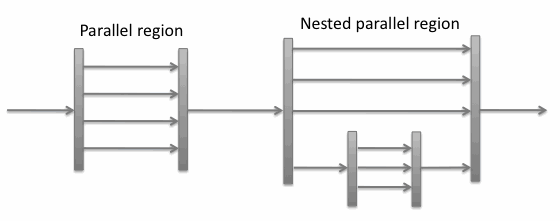
\includegraphics[width=\textwidth]{fork_join}
\captionsetup{justification=centering, singlelinecheck=false}
\caption{Κύριο νήμα και ομάδες νημάτων}
\label{fig:fork_join}
\end{figure}

\clearpage
\subsection{Αλληλεπίδραση νημάτων και περιβάλλοντος δεδομένων}
\subparagraph{}
Η εκτέλεση του προγράμματος ξεκινάει από το κύριο νήμα το οποίο έχει συσχετιστεί με ένα περιβάλλον εκτέλεσης. Το περιβάλλον εκτέλεσης για ένα νήμα είναι ο χώρος διεύθυνσης μνήμης που περιέχει όλες τις μεταβλητές του προγράμματος, περιλαμβανομένων των \en{global} μεταβλητών, των μεταβλητών που είναι αποθηκευμένες στη \en{stack} και αυτών που είναι αποθηκευμένες στη \en{heap}\cite{book2}. 

Στο μοντέλο μνήμης \en{OpenMP}, υπάρχουν δύο διαφορετικοί βασικοί τύποι μνήμης: η ιδιωτική(\en{private}) και η κοινόχρηστη(\en{shared}).  Όλα τα νήματα έχουν πρόσβαση σε μεταβλητές που είναι αποθηκευμένες στην κοινόχρηστη μνήμη\cite{thenextstep7}.

\begin{figure}[h]
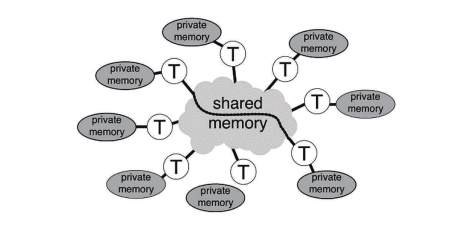
\includegraphics[width=\textwidth]{private_shared}
\captionsetup{justification=centering, singlelinecheck=false}
\caption{Μοντέλο μνήμης \en{OpenMP}}
\label{fig:private_shared}
\end{figure}

\subsubsection{Ιδιωτική μνήμη}
\subparagraph{}
Κάθε νήμα έχει ιδιωτική μνήμη στην οποία έχει πρόσβαση και μπορεί να την τροποποίηση, αλλά δε μπορεί να έχει πρόσβαση στην ιδιωτική μνήμη άλλου νήματος. Η διάρκεια ζωής μιας μεταβλητής στην ιδιωτική μνήμη είναι περιορισμένη και διαρκεί όσο εκτελείται ο παράλληλος κώδικας. Προεπιλεγμένα, η ιδιωτική μεταβλητή δεν είναι αρχικοποιημένη στην αρχή της παράλληλης περιοχής\cite{thenextstep9}.

\clearpage
\subsubsection{Κοινόχρηστη μνήμη}
\subparagraph{}
Εκτός από την ιδιωτική μνήμη, κάθε νήμα έχει πρόσβαση και σε ένα άλλο είδος μνήμης, την  κοινόχρηστη. Σε αντίθεση με την ιδιωτική, υπάρχει μόνο μία κοινόχρηστη μνήμη κατα τη διάρκεια εκτέλεσης του προγράμματος, και είναι προσπελάσιμη απο όλα τα νήματα. Ετσι, κάθε νήμα έχει την δυνατότητα τροποποίησης οποιασδήποτε μεταβλητής βρίσκεται στη κοινόχρηστη μνήμη.
Η ταυτόχρονη προσπέλαση κοινόχρηστης μνήμης από διαφορετικά νήματα, προκαλεί τα παρακάτω προβλήματα:

\paragraph{\en{Race Condition}}

\begin{center}
	\begin{minipage}[t]{0.45\linewidth}
Εμφανίζεται στις περιπτώσεις όπου μια συνάρτηση χρησιμοποιεί δεδομένα από της κοινόχρηστης μνήμης. 
Αν η συνάρτηση καλείται παράλληλα, πολλά νήματα ενδέχεται να τροποποιήσουν ταυτόχρονα την ίδια διεύθυνση μνήμης. Το φαινόμενο αυτό ονομάζεται race condition και η απλούστερη λύση του ειναι η δημιουργία ιδιωτικού αντίγραφου για κάθε νήμα. Με αυτό τον τρόπο, πολλά νήματα μπορούν ταυτόχρονα να τροποποιούν δεδομένα που βρίσκονται σε διαφορετικές θέσεις μνήμης.
	\end{minipage}
	\qquad
	\begin{minipage}[t]{0.47\linewidth}
		\selectlanguage{english}
		\begin{lstlisting}[tabsize=2, basicstyle=\small, language=C++, caption={\el{Παράδειγμα κώδικα με} race condition}, frame=tb]
#include <omp.h>

int main(void) {	
	int sum = 0;

	#pragma omp parallel for
	for (int i = 0;  i < 100; ++i) {
		sum += i;		
	}
}
\end{lstlisting}
\selectlanguage{english}
	\end{minipage}
\end{center}
\clearpage
\paragraph{\en{False Sharing}}
\subparagraph{}
\begin{wrapfigure}{r}{0.6\textwidth} % this figure will be at the right
	\centering
	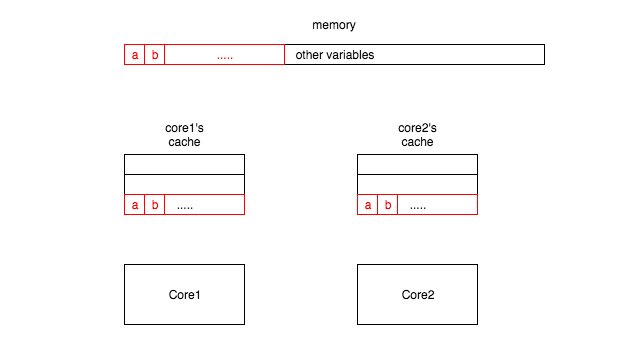
\includegraphics[width=0.6\textwidth]{false_sharing_2}
	\captionsetup{justification=centering, singlelinecheck=false}
	\caption{\en{False sharing (1/3)}}
\label{fig:false_sharing_2}
\end{wrapfigure}

Το \en{false sharing} ειναι ενα συχνό πρόβλημα στην παράλληλη επεξεργασία κοινόχρηστης μνήμης. Εμφανίζεται όταν δυο ή περισσότεροι πυρήνες κρατούν ένα αντίγραφο της ίδιας γραμμής προσωρινής μνήμης. 
\ \\
\ \\
\ \\
\begin{wrapfigure}{l}{0.55\textwidth}
	\centering
	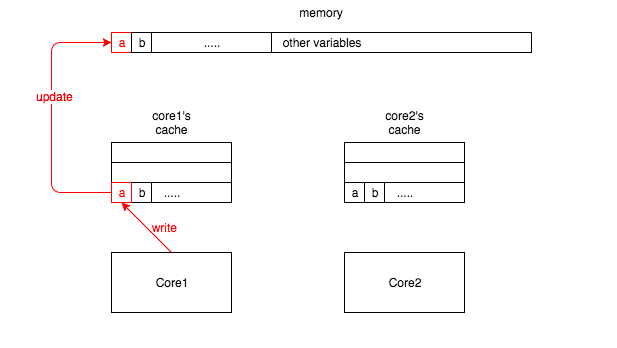
\includegraphics[width=0.55\textwidth]{false_sharing_3}
	\captionsetup{justification=centering, singlelinecheck=false}
	\caption{\en{False sharing (2/3)}}
\label{fig:false_sharing_3}
\end{wrapfigure}

Οταν ένας πυρήνας τροποποιεί μια μεταβλητή, η γραμμή της μνήμης που βρίσκεται η μεταβλητή ακυρώνεται σε άλλους πυρήνες. Παρόλο που ένας πυρήνας μπορεί να μή τροποποιεί της συγκεκριμένη θέση μνήμης, μπορεί να χρησιμοποιεί ένα αλλο στοιχείο δεδομένων στην ίδια γραμμή μνήμης. 
\clearpage
\begin{wrapfigure}{l}{0.6\textwidth}
	\centering
	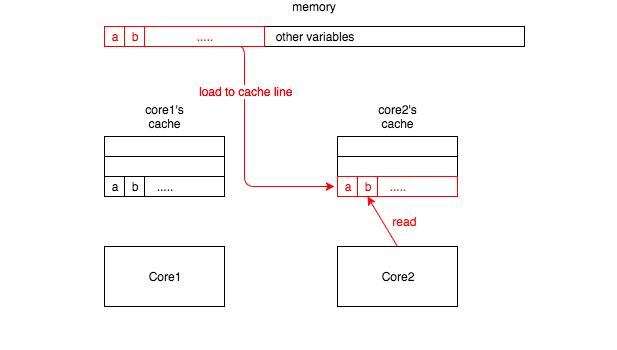
\includegraphics[width=0.6\textwidth]{false_sharing_4}
	\captionsetup{justification=centering, singlelinecheck=false}
	\caption{\en{False sharing (3/3)}}
\label{fig:false_sharing_4}
\end{wrapfigure}
Ο δεύτερος πυρήνας θα πρέπει να φορτώσει εκ νέου τη γραμμή προτού αποκτήσει ξανά πρόσβαση στα δικά της δεδομένα. Η χρήση της κοινόχρηστης μνήμης μπορεί να επηρεάσει την απόδοση του προγράμματος[12].
Λύση στο πρόβλημα του false sharing, αποτελεί η εισαγώγή τεχνιτού κενού (padding) ανάμεσα στα στοιχεία ενός array.

\section{Μεθοδολογία}
\subparagraph{}
Αυτό το μέρος της εργασίας ασχολείται με τον πραγματικό ερευνητικό σχεδιασμό που θα ακολουθηθεί. Μία σύντομη ανασκόπηση των εναλλακτικών λύσεων και των αντίστοιχων πλεονεκτημάτων και μειονεκτημάτων τους θα πρέπει να παρουσιαστεί και η επιλογή μιας συγκεκριμένης προσέγγισης θα πρέπει να εξεταστεί καλά και να συνδεθεί με το(α) πρόβλημα(τα) που εξετάζεται(ονται). Οι δευτερεύουσες και οι βασικές πηγές των στοιχείων θα πρέπει να καθοριστούν και η χρήση τους θα πρέπει να εξεταστεί και να δικαιολογηθεί. Σε έρευνες πεδίου θα πρέπει να διατυπωθούν καθαρά  ο τρόπος συλλογής των στοιχείων, η επιλογή του πληθυσμού που θα ερευνηθεί και η δειγματοληπτική διαδικασία που θα ακολουθηθεί. Οι μετρήσεις που χρησιμοποιήθηκαν θα πρέπει επίσης να δικαιολογηθούν και θα πρέπει να γίνει μια περιγραφή του εργαλείου συλλογής στοιχείων.

Οι εικόνες (και τα σχήματα) εμφανίζονται στο κείμενο όπως παρακάτω. Ο Κατάλογος των Εικόνων ενημερώνεται αυτόματα. Η περιγραφή τους πρέπει να εμφανίζεται κάτω από την εικόνα.



Οι πίνακες εμφανίζονται όπως παρακάτω. Ο Κατάλογος των Πινάκων ενημερώνεται αυτόματα. Η περιγραφή τους πρέπει να είναι πάνω από τον πίνακα.
\begin{table}[htbp]
\captionsetup{justification=raggedright,
singlelinecheck=false
}
\caption{Ένας πίνακας χωρίς νόημα!}
\begin{otherlanguage}{english}
\def\arraystretch{1.5}
\begin{tabular}{| p{2.0cm} | p{2.0cm}| p{2.0cm} | p{2.0cm} | p{2.0cm} |}
\cline{1-5}
A-D & A & B & C & D \\
\cline{1-5}
1 & A1 & B1 & C1 & D1 \\
\cline{1-5}
2 & A2 & B2 & C2 & D2 \\
\cline{1-5}
3 & A3 & B3 & C3 & D3 \\
\cline{1-5}
\end{tabular}
\end{otherlanguage}
\end{table}


\selectlanguage{greek}

\clearpage
\section{Επίλογος}
\subparagraph{}
Εδώ συνοψίζουμε την παρουσίαση της διπλωματικής.

\subsection{Σύνοψη και συμπεράσματα}
\subparagraph{}

Εδώ συνοψίζουμε τα αποτελέσματα της διπλωματικής και περιγράφουμε τα συμπεράσματα που προέκυψαν, αρνητικά και θετικά. Επιβεβαιώνουμε τη συνεισφορά της διπλωματικής στα προβλήματα που αναφέραμε στην εισαγωγή. Τα συμπεράσματα θα πρέπει να παρουσιάζονται συστηματικά για κάθε αντικειμενικό στόχο ή υπόθεση που έχουμε κάνει.

\subsection{Όρια και περιορισμοί της έρευνας}
\subsection{Μελλοντικές Επεκτάσεις}
\subparagraph{}
Εδώ δίνουμε ιδέες για επέκταση της διπλωματικής. Αναφέρουμε ότι θα ακολουθήσει παρουσίαση μελλοντικών κατευθύνσεων έρευνας ανά θεματική περιοχή. Περιγράφουμε προβλήματα που δεν έχουν λυθεί από τις τεχνικές/μεθοδολογίες που παρουσιάσαμε στο προηγούμενο κεφάλαιο. Τα άλυτα αυτά προβλήματα, αποτελούν στην ουσία προκλήσεις για περαιτέρω έρευνα. Ακόμα καλύτερα, θα ήταν ωραία να προτείνουμε τρόπους επίλυσης των προβλημάτων αυτών έστω και ως γενική ιδέα.

\clearpage
\selectlanguage{greek}

 \selectlanguage{english}
 \bibliography{bibliogr.bib}
 \bibliographystyle{abbrv}
\end{document}